The Chan-Vese algorithm is an active contour method. In active contour methods, the goal is to minimise an energy along a curve, by evolving that curve in a descent direction for the energy. Energy is computed on image data and curve's regularity.
Many models exist for the curve energy. The Chan-Vese model has the advantage to not be based on edge detection, so can detect objects without distinct edges.

\subsection{The Chan-Vese model for the energy}

The energy to minimise in Chan-Vese method is :
\begin{equation}
\begin{split}
F(c_1,c_2,C)& = \alpha . \text{Length}(C) + \beta . \text{Area}(inside(C)) \\
            & \quad + \lambda_1.\int_{inside(C)} |u_0(x,y) - c_1| dx dy \\
            & \quad - \lambda_2.\int_{outside(C)} |u_0(x,y) - c_2| dx dy
\label{cv_energy}
\end{split}
\end{equation}

Where $C$ is a closed curve (which should fit the target object), $u_0$ is the gray level function from the picture, $c_1$, $c_2$ respectively the inner and outter gray level means. 

The term $\alpha.\text{Length}(C)$ ensure smooth of the curve, as we minimise its length. $\beta . \text{Area}(inside(C))$ is also about regularity. 

The term $ \lambda_1.\int_{inside(C)} |u_0(x,y) - c_1| dx dy - \lambda_2.\int_{outside(C)} |u_0(x,y) - c_2| dx dy$ should be minimum when the curve fits at best the object. An intuitive way to see it : for an monochromatic object on an monochromatic background, this term will be null if the curve fit the object.

\subsection{Minimise the energy}

This part is mathematical. It aims to exhibit a way to minimise F algorithmically.

We need a way to calculate C. So we redefine C implicitly by $\phi : \mathbb{R}^2 \rightarrow \mathbb{R}$ such that : \\

    \phi = \begin{cases}
     0& (x,y) \in C \\
     <0& (x,y) \in outside(C) \\
     >0& (x,y) \in inside(C)
     \end{cases}
    
\\
\\
 Then we can write the energy F :

\begin{equation}
\begin{split}
F(c_1,c_2,C)& = \alpha . \int_{\Omega} \delta_0 (\phi(x,y)) |\bigtriangledown \phi(x,y)| dxdy + \beta . \int_{\Omega} H(\phi(x,y))dxdy \\
            & \quad + \lambda_1.\int_{\Omega} |u_0(x,y) - c_1| H(\phi(x,y)) dx dy \\
            & \quad - \lambda_2.\int_{\Omega} |u_0(x,y) - c_2|(1-H(\phi(x,y))) dx dy
\end{split}
\end{equation}

Where $H$ is the Heaviside function and $\delta_0$ the Dirac distribution.

Both function are regularised, respectively by $H_\epsilon$ and $\delta_\epsilon$ (in the algorithm we need only to compute $\delta_\epsilon$ which is done by taking a narrow band around $\phi$)

This formulation allows us to apply Euler-Lagrange equation, which give F derivative relatively to $\phi$

So we have a descent direction for $\phi$. Parameterising $\phi$ descent by $t$, we get :

\begin{equation}
\frac{\partial \phi}{\partial t} = \delta_\epsilon(\phi)\left[ \mu . div \left( \frac{\bigtriangledown \phi(x,y)}{|\bigtriangledown \phi(x,y)| \right)  - \nu + \lambda_1 (u_0 - c_1)^2 - \lambda_2 (u_0 - c_2)^2 \right] }
\label{descent_direction}
\end{equation}

For more details see [1].


\subsection{Algorithm, stopping criterion}

The algorithm is then the following :
\begin{itemize}
\item Initialize $\phi$
\item Compute $c_1$ and $c_2$
\item Iterate $\phi$ in descent direction
\item If convergenced then stop else go back to second step
\end{itemize}

As the algorithm is actually a conjugate gradient one, we could check the convergence by checking stationnarity of $\phi$.
Though it appears that at convergence $\phi$ slighty oscillate.

\begin{figure}[H]
\centering
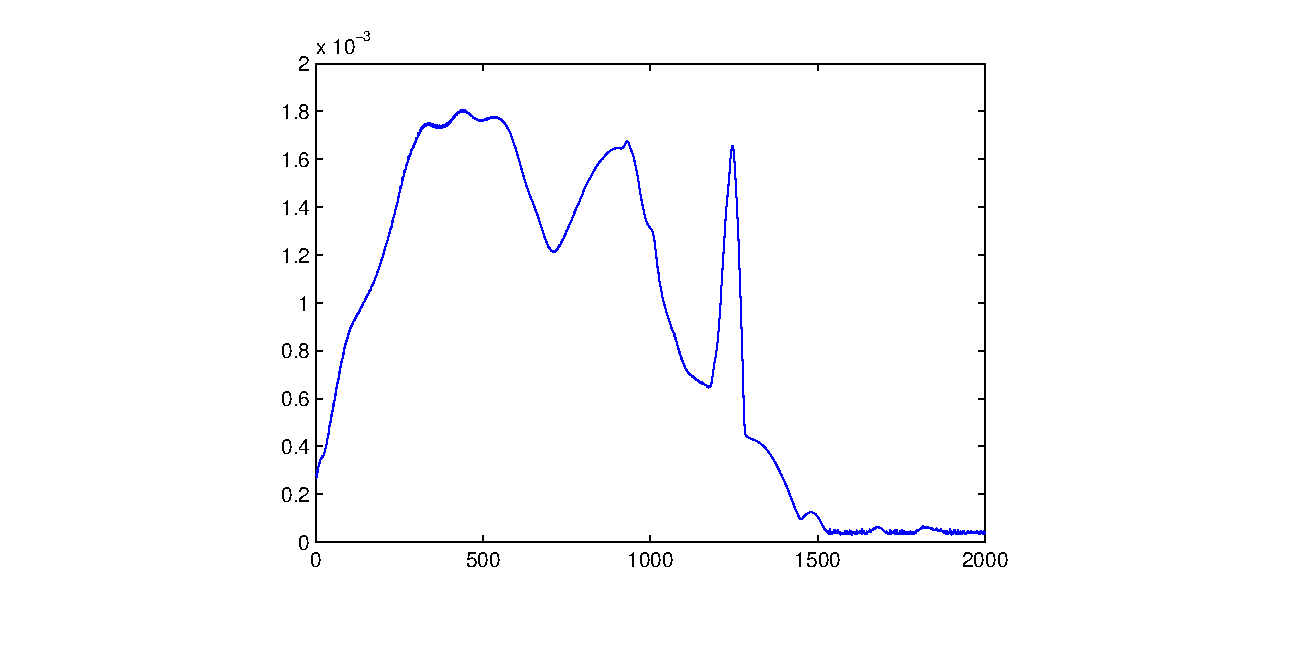
\includegraphics[scale=0.7]{images/crit_it_rx1_t1.eps}
\caption{$||{\phi_{n+1}-\phi_n}||$ according to the number of iteration, for rx1 picture}
\label{fig1}
\end{figure}

\begin{figure}[H]
\centering
\includegraphics[scale=0.7]{images/crit_it_rx2_t1_zoom.eps}
\caption{$||{\phi_{n+1}-\phi_n}||$ according to the number of iteration, for rx1 picture}
\label{fig2}
\end{figure}

$S_1 = ||{\phi_{n+1}-\phi_n}||$ can't be taken as a stopping criterion. This value stabilise at around $10^-4$ for rx1 (see figure~\ref{fig1}), $10^-5$ for rx2 (see figure~\ref{fig2}). So it is hard to define a tolerance.
Then we decided to choose as a stopping criterion the derivative of $S_1$, filter by a low pass filter (to suppress oscillation effect, see figure~\ref{fig3}). The algorithm stop if $\frac {dS_1} {dn} < tol$ over 20 iterations. 
Oscillations can be explain by the fact that $c_1$ and $c_2$ depends on $\phi$, but doesn't appear in descent term, so a sightl error is introduced which prevent the algorithm to totally stabilise.

\begin{figure}[H]
\centering
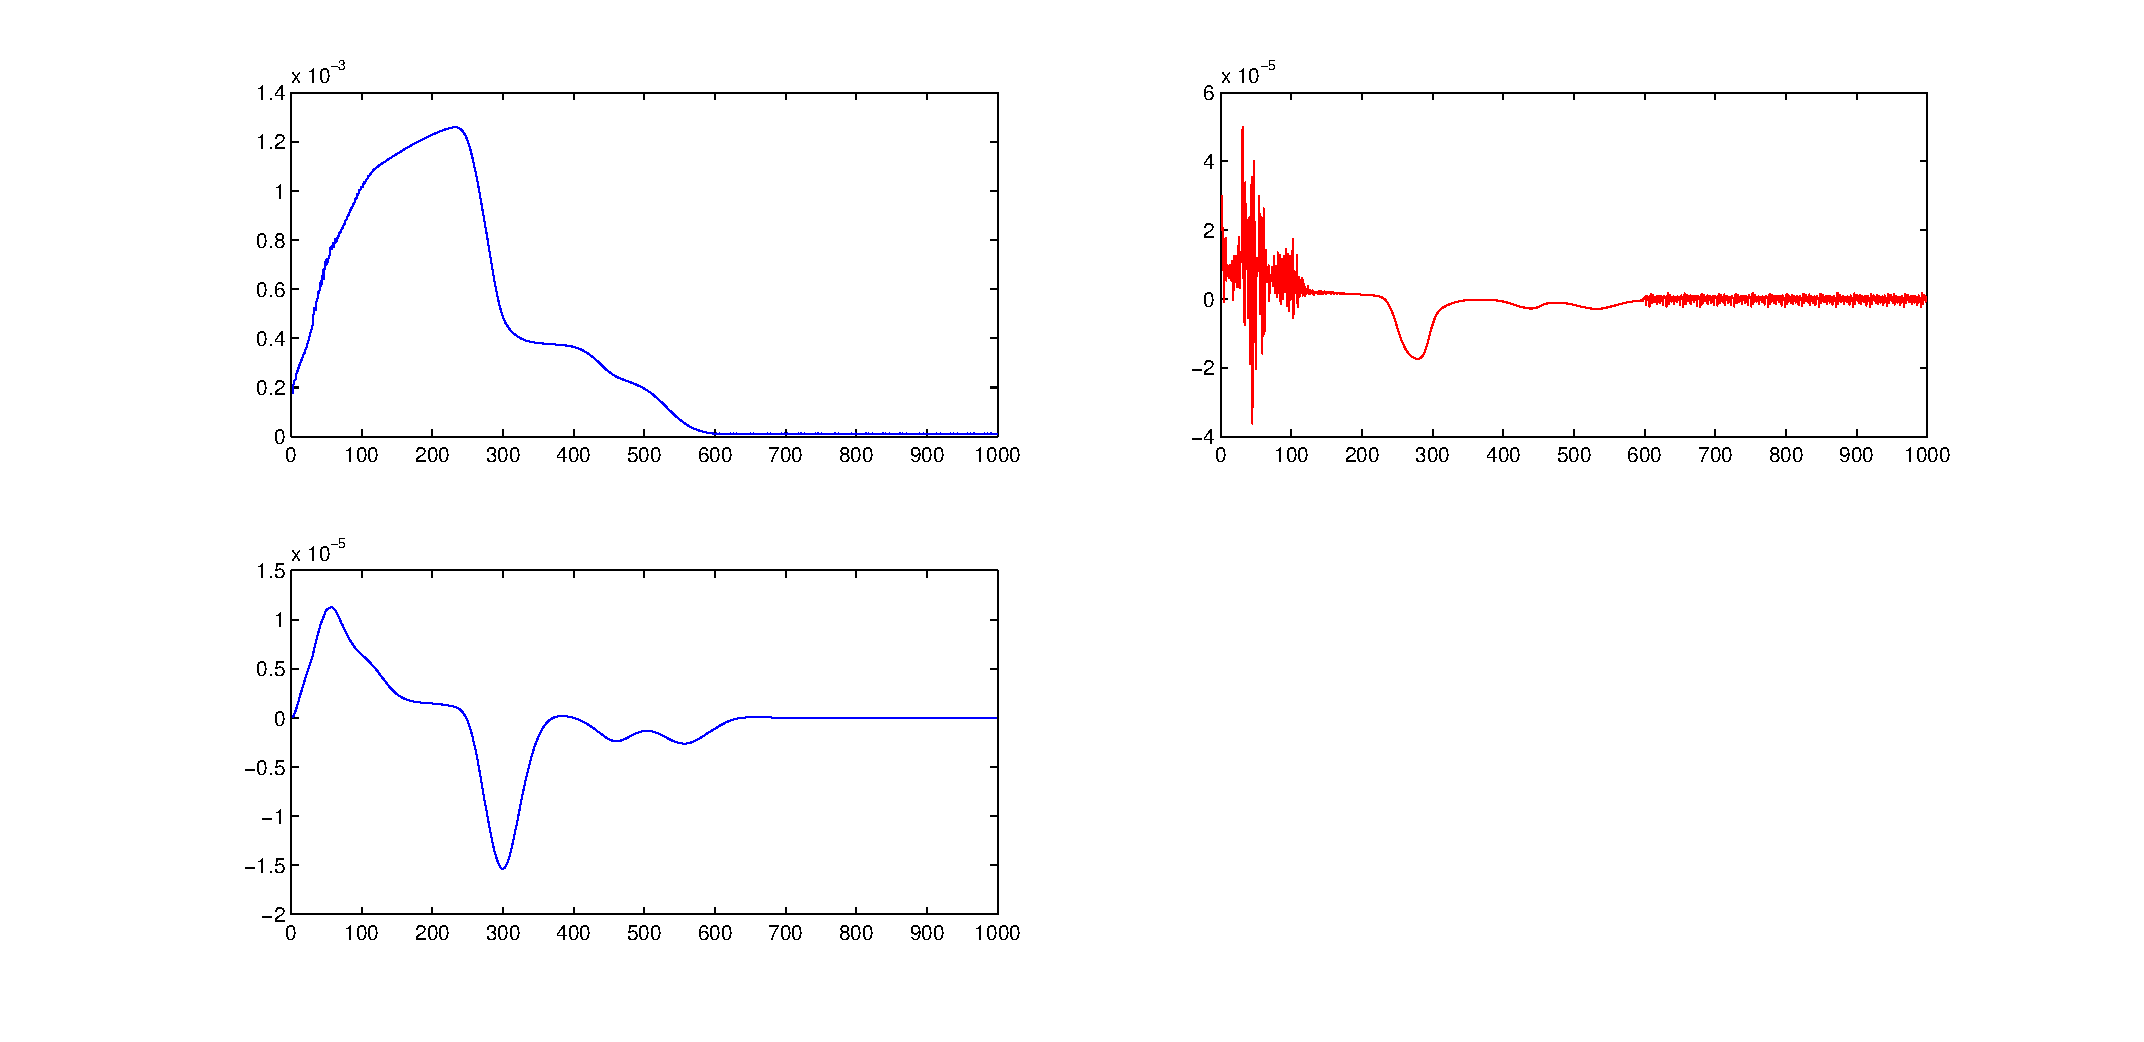
\includegraphics[scale=0.4]{images/crit_it_rx2_t2.eps}
\caption{From left to right : $S_1$, its derivative, and its filtered derivative}
\label{fig3}
\end{figure}

\subsection{Tests}

As Euler-Lagrange equation can only ensure a local minimum, the algorithm depends on initialisation.
It also depends on coefficients $\alpha$ relative to $\lamba_1$ and $\lambda_2$. We set $\lambda_2 = 1$ for the tests.
Figures % TO COMPLETE 
in annexes shows the result depends on whole parameters.
Moreover goods results may be obtain for different parameters on two pictures.
The work to be described further is try to automatise the algorithm (reduce or even suppress the parameters dependency).

\subsection{Local segmentation}
\textit{See section \ref{localcode} for the \texttt{MatLab} code}.\\
A way to really improve the active contour method for more heterogeneous picture, like radiography, is to use local statistics instead of global statistics in the algorithm. Indeed, we can see in figure \ref{interestLocal} that the bottom of the tooth has almost the same shade of gray than some part of the gum. So the global method won't be able to distinguish those two parts of the radiography. The key here is to not examine those two parts together, and instead, examine each pixel of the radiography locally. In other words, at each iteration of the algorithm, instead of having statistics about the whole picture, we create a small ball centred on the current pixel and calculate the same statistics but inside the ball. For further information, see \cite{lanktonLO}. 

\begin{figure}[H]
\centering
\includegraphics[scale=1.8]{images/rx1.png}
\caption{Interest of the local active contour method : bottom of the tooth has the same shade of gray as some part of the gum}
\label{interestLocal}
\end{figure}

In the following (see the next two figures), we create another initialisation for the active contour method by using two ellipses, one around the tooth and one between the two roots. So that if we take the area between the two ellipses, we can have a pretty good initialisation. Here is an example of the improvement brought by the local method compared to the global method (we used the exact same parameter and the same number of iteration): 
\begin{figure}[H]
\centering
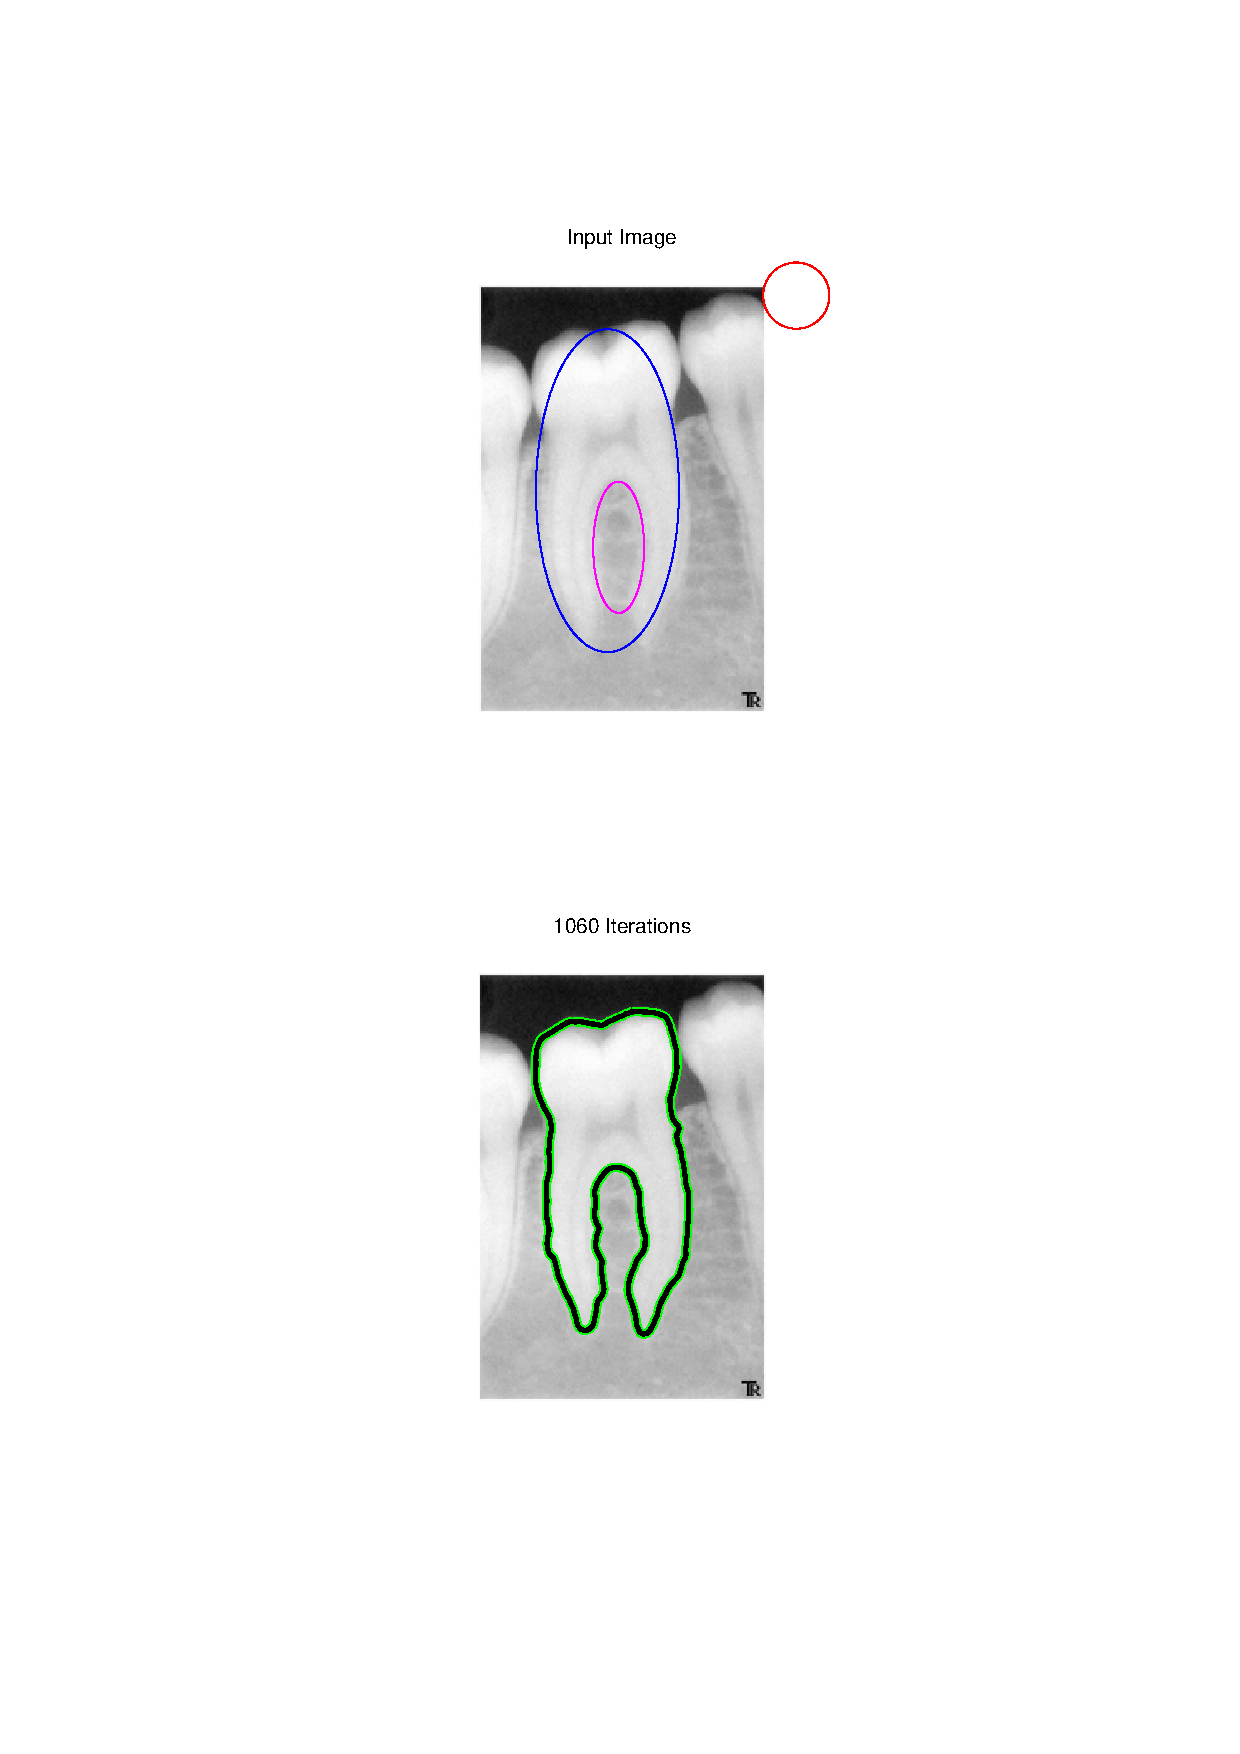
\includegraphics[scale=0.8]{images/doubleEllipseTest_rx2.png}
\caption{Segmentation with the local method : Red circle has the same radius as the ball used in the algorithm. The two ellipses are used for the initialisation.}
\label{ellipseLO}
\end{figure}
As we can see, the segmentation is here almost perfect with the local algorithm. Segmentation with the region based active contour method is behaving as expected : since the tooth shade of gray is almost the same as the gum, the algorithm cannot separate them (see figure \ref{ellipseGLO}). However, local algorithm is really slow since we have to consider each pixel around the zero level set of $\phi$ and calculate statistics of pixels in the ball centred on the first pixel. The total execution time of the local algorithm was about 20 minutes on this high definition radiography while the global method execution time was barely 30 seconds. To improve the local algorithm, we have to use another way to implement the level set function $\phi$. The best is the sparse field method proposed by Whitaker (see \cite{whitaker} for more details). The author of \cite{lanktonLO} implemented this method on the local algorithm and it did save a lot of computations (see \cite{lanktonSFM}).     
\begin{figure}[H]
\centering
\includegraphics[scale=0.8]{images/doubleEllipseTest_rx2_region.png}
\caption{Segmentation with the global method : bad segmentation between the two teeth.}
\end{figure}



